\documentclass[9pt]{beamer}

\usepackage[T1]{fontenc}
\usepackage{color}
\usepackage{graphicx}
\usepackage{natbib}
\usepackage{tikz}
\usepackage{xmpmulti}
\usepackage{animate}

\usetheme{Boadilla}

\usefonttheme{professionalfonts}

\title[Apsis Tools]{Apsis - Big literature tools and methods}
\subtitle{}
\author{Max Callaghan}
\institute[MCC]{
	%
\includegraphics[height=1cm,width=2cm]{/home/max/Pictures/MCC_Logo_RZ_rgb.jpg}
	
\includegraphics[height=1cm,width=2cm]{MCC_Logo_RZ_rgb.jpg}
}

\usetikzlibrary{shapes.geometric, arrows}
\tikzstyle{startstop} = [rectangle, rounded corners, minimum width=2.5cm, minimum height=1cm,text centered, draw=black, text width=2.5cm, fill=red!30]
\tikzstyle{product} = [rectangle, rounded corners, minimum width=2.5cm, minimum height=1cm,text centered, draw=black, text width=2.5cm, fill=cyan!30]
\tikzstyle{process} = [rectangle, minimum width=2cm, text width=2cm, minimum height=1cm, text centered, draw=black, fill=orange!30]
\tikzstyle{person} = [ellipse, minimum width=2cm, text width=2cm, minimum height=1cm, text centered, draw=black, fill=green!30]
\tikzstyle{io} = [trapezium, trapezium left angle=70, trapezium right angle=110, minimum width=1cm, minimum height=1cm, text centered, draw=black, fill=blue!30, inner sep=10]

\tikzstyle{label} = [rectangle, minimum width=0.8cm, minimum height=0.8cm, text centered, draw=black, fill=blue!0, inner sep=3]

\tikzstyle{arrow} = [thick,->,>=stealth]


\newtheorem*{remark}{}

\bibliographystyle{apalike}

\begin{document}
	
\begin{frame}
	\titlepage
\end{frame}

\addtobeamertemplate{frametitle}{}{%
	\begin{tikzpicture}[remember picture,overlay]
	\node[anchor=north east,yshift=2pt] at (current page.north east) {
\includegraphics[height=0.8cm]{MCC_Logo_RZ_rgb.jpg}};
	\end{tikzpicture}}

\begin{frame}{Infrastructure}
	\begin{center}
	\def\yspace{1.5cm}
	\resizebox{0.9\linewidth}{!}{
		\begin{tikzpicture}[node distance=3cm]
		\node (Data) [startstop] {Data Collection};
		\node (Analysis) [startstop, right of=Data, node distance=6cm] {Analysis};
		\node (Presentation) [startstop, right of=Analysis, node distance=6cm] {Presentation};
		
		\node (WoS) [process, below of=Data, node distance=1.8cm, xshift=-2cm] {WoS};
		\node (Scopus) [process, below of=WoS, node distance=\yspace] {Scopus};
		\node (IPCC) [process, below of=Scopus, node distance=\yspace] {IPCC};
		\node (Consolidation) [io, right of=Scopus, node distance=3.5cm] {Consolidation};
		
		\node (Manual) [label, below of=Analysis, node distance=1.8cm, xshift=-1.2cm] {Manual};
		\node (Automatic) [label, below of=Manual, node distance=4.5cm] {Automatic};
		
		
		\node (Review) [process, below of=Analysis, node distance=1.8cm, xshift=1cm] {Systematic Review};
		\node (Scientometric) [process, below of=Review, node distance=\yspace] {Scientometric Analysis};
		\node (Text) [process, below of=Scientometric, node distance=\yspace, fill=orange!15] {Text Analysis};
		\node (Topics) [process, below of=Text, node distance=\yspace] {Topic Modelling};
		
		\node (Plots) [process, below of=Presentation, node distance=1.8cm, xshift=0cm] {Plots};
		\node (Tables) [process, below of=Plots, node distance=\yspace] {Tables};
		\node (Online) [process, below of=Tables, node distance=\yspace] {Online Explorer};
		
		
		\node (Database) [product, below of=Data, node distance=9cm] {Database};
		
		\node (Analysis) [product, below of=Analysis, text width=5cm, node distance=9cm] {Scoping Platform; \\ Rstudio Server; \\ Jupyter Notebooks};
			
		\node (Server) [product, below of=Presentation, text width=3cm, node distance=9cm] {Web server};
		
		
		\draw [arrow] (Manual) -- (Automatic);
		
		\end{tikzpicture}
	}
\end{center}
\end{frame}

\begin{frame}{}

\begin{columns}
	\begin{column}{0.5\linewidth}
		\begin{center}
			\begin{figure}
				%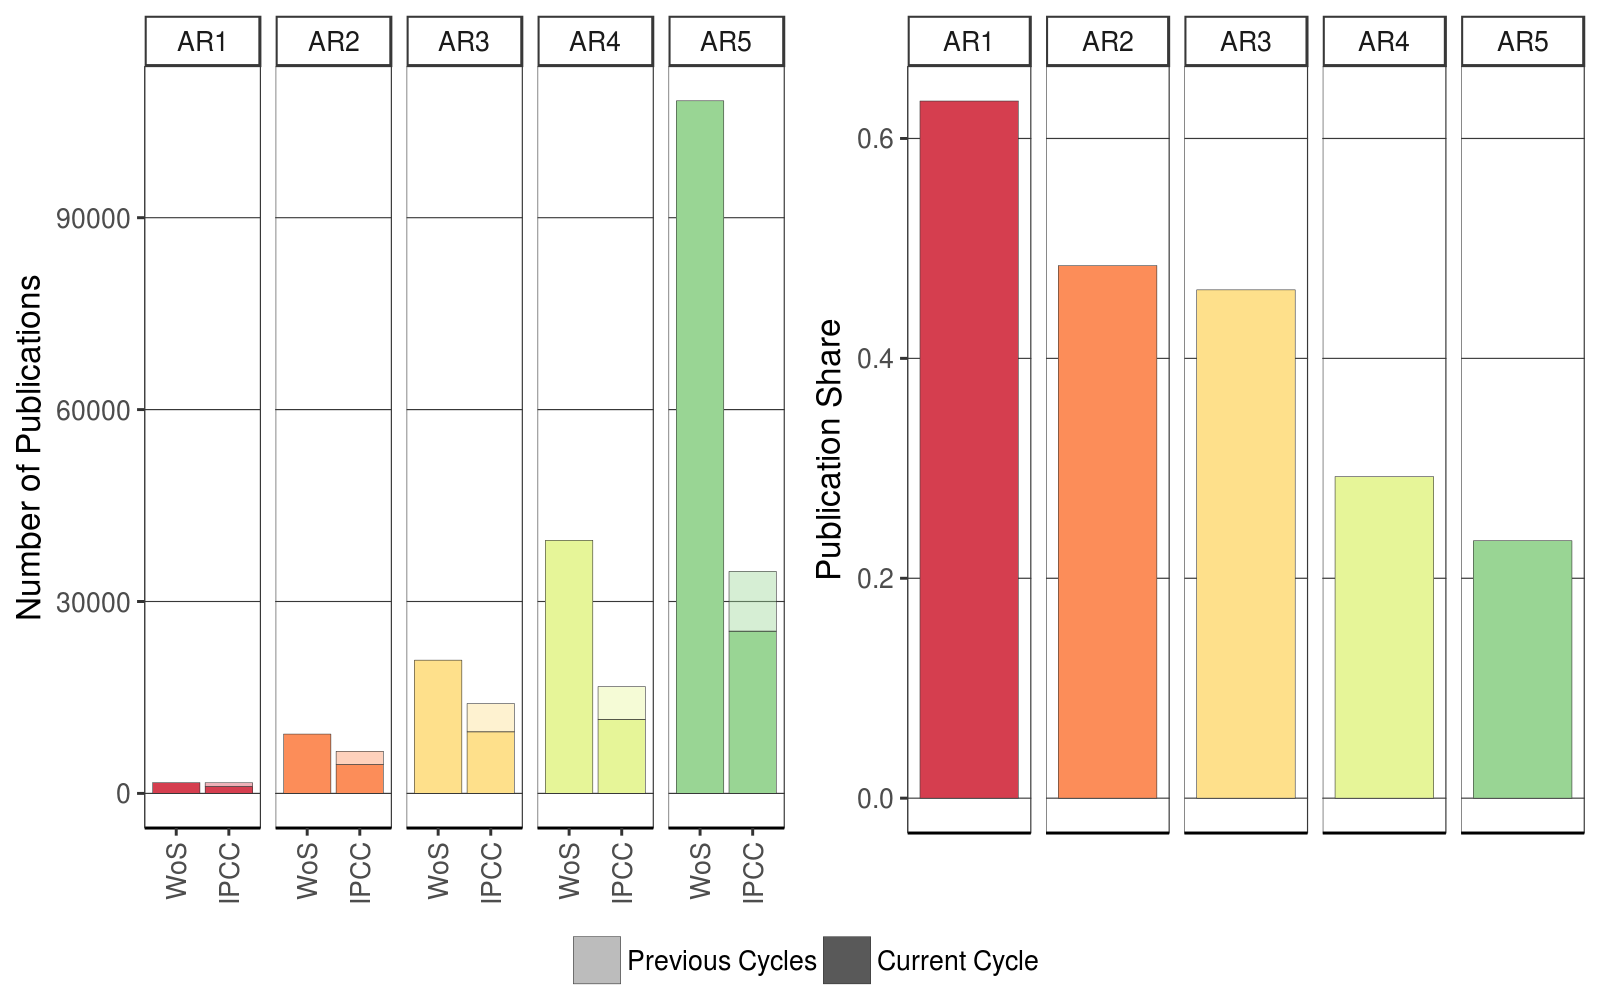
\includegraphics[width=0.85\linewidth]{merged_IPCC_spectral.png}
			%	\caption{Source: \citet{Minx2017} }
		\animategraphics[loop,controls,width=\linewidth]{12}{images/screen-}{0}{248}
			\end{figure}
		\end{center}
	\end{column}
	\begin{column}{0.5\linewidth}
		\begin{center}
			\begin{itemize}
				\item Comprehensive, credible and relevant assessments become
				more challenging as the literature grows
			\end{itemize}
		\end{center}
	\end{column}
\end{columns}

\end{frame}

\begin{frame}{Frame Title}
	\small
	%\bibliography{/home/max/Documents/library/bibliography}
	\bibliography{C:/Users/galm/Documents/library/library}
\end{frame}

\end{document}
